\documentclass[11pt,letterpaper]{article}

% Packages
\usepackage[utf8]{inputenc}
\usepackage[T1]{fontenc}
\usepackage{amsmath,amssymb,amsthm}
\usepackage{algorithm}
\usepackage{algorithmic}
\usepackage{graphicx}
\usepackage{hyperref}
\usepackage{xcolor}
\usepackage{booktabs}
\usepackage{tikz}
\usetikzlibrary{shapes,arrows,positioning}
\usepackage{listings}
\usepackage{caption}
\usepackage{subcaption}

% Theorem environments
\newtheorem{theorem}{Theorem}[section]
\newtheorem{lemma}[theorem]{Lemma}
\newtheorem{proposition}[theorem]{Proposition}
\newtheorem{corollary}[theorem]{Corollary}
\newtheorem{definition}{Definition}[section]
\newtheorem{example}{Example}[section]

% Custom commands
\newcommand{\Zoo}{\textsc{Zoo}}
\newcommand{\HLLM}{\textsc{hllm}}
\newcommand{\DSO}{\textsc{dso}}
\newcommand{\DAO}{\textsc{dao}}
\newcommand{\IPFS}{\textsc{ipfs}}
\newcommand{\LLM}{\textsc{llm}}

% Hyperref setup
\hypersetup{
    colorlinks=true,
    linkcolor=blue,
    citecolor=blue,
    urlcolor=blue
}

% Title and authors
\title{\textbf{Experience Ledger: Decentralized Semantic Optimization for Large Language Models}\\
\large Version 2025.09}

\author{
Zoo Labs Foundation Inc\\
\texttt{research@zoo.ngo}\\
\\
\textit{A 501(c)(3) Non-Profit Organization}
}

\date{September 2025}

\begin{document}

\maketitle

\begin{abstract}
We present the \textit{Experience Ledger}, a decentralized infrastructure for semantic optimization of Large Language Models (\LLM{}s) that replaces centralized fine-tuning with community-driven knowledge curation. Unlike traditional approaches that update model parameters—an opaque, expensive, and centralized process—our system maintains a content-addressable library of semantic advantages: natural language insights extracted via introspection that guide model behavior through context injection. The Experience Ledger combines cryptographic verification (Merkle trees), decentralized storage (\IPFS{}/Arweave), and \DAO{}-based governance to enable transparent, auditable, and democratic model evolution. We demonstrate that semantic optimization achieves comparable or superior performance to parameter fine-tuning at 0.2\% of the cost while enabling cross-domain transfer, interpretability, and Byzantine-robust aggregation. This paradigm shift—from implicit weight updates to explicit wisdom commons—establishes a foundation for truly decentralized artificial intelligence.
\end{abstract}

\section{Introduction}

The democratization of artificial intelligence remains an unfulfilled promise. While open-source Large Language Models (\LLM{}s) have proliferated, their effective deployment requires fine-tuning—a process dominated by well-resourced institutions with access to specialized hardware, proprietary datasets, and ML engineering expertise. This centralization creates multiple failure modes: opaque model behavior, catastrophic forgetting across domains, high computational costs (\$10,000+ per task), and the impossibility of community-driven model evolution.

Consider the typical fine-tuning workflow: A research lab collects thousands of task-specific examples, performs gradient-based parameter updates over days of GPU time, and publishes the resulting model weights. Users must trust that the updates improve performance without introducing biases or vulnerabilities. If the model fails on edge cases, there is no mechanism for incremental correction beyond complete retraining. Cross-domain applications require separate fine-tuned variants, fragmenting the ecosystem. Most critically, the knowledge encoded during fine-tuning remains locked within billions of parameters—inaccessible to inspection, debate, or collaborative refinement.

\subsection{The Alchemical Transformation}

We propose a radical alternative: \textit{Decentralized Semantic Optimization} (\DSO{}). Rather than transmuting model parameters through gradient descent—a black-box process akin to medieval alchemy's futile pursuit of metallic transformation—we extract and curate \textit{semantic advantages}: explicit, human-readable insights that capture effective reasoning patterns. These experiences form a public knowledge commons, verified through cryptography, stored via decentralized protocols, and governed by community consensus.

The Experience Ledger serves as the philosophical stone of this transformation, converting the base metal of raw computational trajectories into the gold of distilled wisdom. Each experience represents a crystallized insight—"When solving geometry problems with intersections, validate solutions lie within bounded regions, not on extensions"—that can be inspected, debated, improved, and composed with others. The model itself remains frozen, a universal reasoning engine, while its behavior adapts through the accretion of verified experiences.

\subsection{Core Contributions}

This paper establishes the theoretical foundations and practical implementation of the Experience Ledger:

\begin{enumerate}
    \item \textbf{Semantic Advantage Format}: A rigorous specification for encoding reasoning insights as natural language statements with cryptographic commitments (Section~\ref{sec:format}).
    
    \item \textbf{Three-Layer Storage Architecture}: Integration of on-chain Merkle roots (\Zoo{} Network L2), mutable content-addressing (\IPFS{}), and permanent archival (Arweave) that balances efficiency, verifiability, and permanence (Section~\ref{sec:storage}).
    
    \item \textbf{Embedding-Based Retrieval}: A 7680-dimensional semantic space enabling sub-linear retrieval of relevant experiences via cosine similarity, with provable coverage guarantees (Section~\ref{sec:retrieval}).
    
    \item \textbf{\DAO{}-Based Curation Protocol}: Game-theoretic mechanisms for Byzantine-robust aggregation of community improvements, including reputation systems and quadratic voting (Section~\ref{sec:curation}).
    
    \item \textbf{\DSO{} Algorithm}: Formal specification of Add/Modify/Delete operations with convergence proofs and conflict resolution strategies (Section~\ref{sec:dso}).
    
    \item \textbf{Empirical Validation}: Comparative evaluation against fine-tuning, RLHF, and prompt engineering across mathematical reasoning (AIME) and web navigation (WebWalker) tasks, demonstrating 99.8\% cost reduction and superior cross-domain transfer (Section~\ref{sec:evaluation}).
\end{enumerate}

The Experience Ledger is not merely a technical system but a \textit{political} architecture—a democratic alternative to AI feudalism where model capabilities are controlled by those with capital. By making knowledge explicit, cryptographically verifiable, and collectively owned, we enable true AI commons.

\section{Background and Related Work}

\subsection{The Limitations of Parameter Fine-Tuning}

Traditional \LLM{} fine-tuning operates in parameter space $\Theta \in \mathbb{R}^d$ (where $d \approx 10^{9}$--$10^{12}$). Given a base model $\pi_{\theta_0}$ and task-specific dataset $\mathcal{D} = \{(x_i, y_i)\}_{i=1}^N$, the objective is:

\begin{equation}
\theta^* = \arg\min_{\theta} \mathbb{E}_{(x,y) \sim \mathcal{D}}[\mathcal{L}(\pi_\theta(x), y)] + \lambda \|\theta - \theta_0\|^2
\end{equation}

This approach suffers from fundamental limitations:

\begin{itemize}
    \item \textbf{Opacity}: Changes to billions of parameters are uninterpretable.
    \item \textbf{Catastrophic Forgetting}: Updates for task A degrade performance on task B.
    \item \textbf{Computational Cost}: Requires 20,000+ GPU-hours (\$10,000+) for 32B models.
    \item \textbf{Centralization}: Only well-funded labs can afford iterative refinement.
    \item \textbf{Non-Composability}: Cannot combine task-specific fine-tunes without retraining.
    \item \textbf{Lack of Provenance}: No audit trail for why parameters changed.
\end{itemize}

\subsection{Reinforcement Learning from Human Feedback (RLHF)}

RLHF methods~\cite{christiano2017deep,ouyang2022training} improve upon supervised fine-tuning by learning from preference data:

\begin{equation}
\mathcal{L}_{\text{RLHF}}(\theta) = \mathbb{E}_{x \sim \mathcal{D}}[r_\phi(\pi_\theta(x))] - \beta \text{KL}(\pi_\theta || \pi_{\text{ref}})
\end{equation}

where $r_\phi$ is a learned reward model and $\beta$ controls divergence from reference policy $\pi_{\text{ref}}$. Recent variants include:

\begin{itemize}
    \item \textbf{PPO}~\cite{schulman2017proximal}: Proximal Policy Optimization with value networks
    \item \textbf{DPO}~\cite{rafailov2023direct}: Direct Preference Optimization (value-free)
    \item \textbf{GRPO}~\cite{shao2024deepseekmath}: Group Relative Policy Optimization
\end{itemize}

While RLHF reduces reliance on labeled data, it still updates parameters and inherits all aforementioned limitations. The reward model $r_\phi$ is itself a black box, and the optimization process lacks transparency.

\subsection{Prompt Engineering and RAG}

An alternative paradigm operates in \textit{context space} rather than parameter space. Prompt engineering manually crafts instructions, while Retrieval-Augmented Generation (RAG)~\cite{lewis2020retrieval} dynamically retrieves relevant documents:

\begin{equation}
\pi_\theta(y | x) = \mathbb{E}_{d \sim \text{Retrieve}(x, \mathcal{D})}[\pi_\theta(y | x, d)]
\end{equation}

RAG maintains model parameters fixed ($\theta = \theta_0$) while augmenting context. However:

\begin{itemize}
    \item Retrieval targets \textit{factual} content, not \textit{reasoning strategies}
    \item No mechanism for extracting insights from model's own trajectories
    \item Quality depends on external document corpus, not learned experiences
\end{itemize}

\subsection{Training-Free Optimization}

Recent work demonstrates LLMs can "learn" via context manipulation:

\begin{itemize}
    \item \textbf{In-Context Learning}~\cite{brown2020language}: Few-shot examples as context
    \item \textbf{Chain-of-Thought}~\cite{wei2022chain}: Step-by-step reasoning prompts
    \item \textbf{Tree-of-Thoughts}~\cite{yao2023tree}: Exploring multiple reasoning paths
    \item \textbf{Self-Consistency}~\cite{wang2022self}: Sampling diverse solutions and voting
\end{itemize}

Our work extends this paradigm by:
\begin{enumerate}
    \item Automatically extracting reasoning strategies via introspection
    \item Accumulating insights across training epochs (not ephemeral per-query)
    \item Decentralizing curation through blockchain governance
\end{enumerate}

Training-Free GRPO~\cite{tencentyoutu2025grpo} pioneered semantic advantage extraction but lacked decentralized infrastructure. The Experience Ledger provides the missing cryptographic and governance layers.

\subsection{Decentralized Machine Learning}

Prior work on decentralized ML~\cite{mcmahan2017communication,kairouz2021advances} focuses on federated learning: training models across distributed devices while preserving privacy. Key differences from our approach:

\begin{itemize}
    \item Federated learning still updates parameters (just distributed)
    \item Goal is privacy-preserving aggregation of gradients, not knowledge curation
    \item No concept of semantic experiences or interpretable improvements
\end{itemize}

Blockchain-based ML systems~\cite{kurtulmus2018trustless,harris2019decentralized} have explored on-chain model verification and compute marketplaces but do not address the semantic optimization problem.

\section{Experience Format Specification}
\label{sec:format}

\subsection{Semantic Advantage Definition}

\begin{definition}[Semantic Advantage]
A semantic advantage is a natural language statement $e \in \mathcal{E}$ that encodes a generalizable reasoning pattern extracted from comparative analysis of model trajectories. Formally, $e$ consists of:

\begin{itemize}
    \item \textbf{Text} $e.\text{text} \in \Sigma^*$: The insight itself (max 32 words)
    \item \textbf{Domain} $e.\text{domain} \in \mathcal{D}$: Problem category (e.g., "math.geometry")
    \item \textbf{Confidence} $e.\text{conf} \in [0,1]$: Quality score derived from advantage magnitude
    \item \textbf{Embedding} $e.\text{emb} \in \mathbb{R}^{7680}$: Semantic vector for retrieval
    \item \textbf{Metadata} $e.\text{meta}$: Creation timestamp, author, usage statistics
\end{itemize}
\end{definition}

\subsection{JSON Schema}

The canonical representation uses JSON with content-addressable identifiers:

\begin{lstlisting}[language=json,caption=Experience JSON Schema,label=lst:schema]
{
  "id": "exp_sha256_abc123...",
  "version": "1.0",
  "domain": "math.geometry",
  "text": "When solving geometry problems with 
           intersections, validate solutions lie 
           within bounded regions, not extensions.",
  "confidence": 0.87,
  "examples": [
    {
      "input": "Find intersection of line AB...",
      "output": "Point P lies outside segment AB...",
      "correct": false
    },
    {
      "input": "Find intersection within triangle...",
      "output": "Point Q is at (3,4) inside ABC.",
      "correct": true
    }
  ],
  "metadata": {
    "created_at": "2025-09-15T14:30:00Z",
    "created_by": "0x742d35Cc6634C0532925a...",
    "votes": {"upvotes": 24, "downvotes": 2},
    "usage_count": 156,
    "domains_applied": ["geometry", "optimization"]
  },
  "embedding": [0.123, -0.456, ...],  // 7680-dim
  "merkle_proof": "0xdef456..."
}
\end{lstlisting}

\subsection{Constraints and Validation}

Valid experiences must satisfy:

\begin{enumerate}
    \item \textbf{Length}: $|e.\text{text}| \leq 32$ words (enforced via tokenization)
    \item \textbf{Structure}: "When [context], [action]" or "[precondition] implies [strategy]"
    \item \textbf{Generality}: No problem-specific constants (e.g., "solve $x^2 = 4$" is invalid)
    \item \textbf{Actionability}: Must guide reasoning, not merely state facts
    \item \textbf{Non-Redundancy}: $\forall e' \in \mathcal{E}, \cos(e.\text{emb}, e'.\text{emb}) < 0.9$
\end{enumerate}

\subsection{Example Experience Library}

\begin{example}[Mathematical Reasoning Experiences]
\begin{enumerate}
    \item \texttt{[G0]} "When solving geometry problems with intersections, validate solutions lie within bounded regions or segments, not on extensions, to avoid extraneous answers."
    
    \item \texttt{[G1]} "For expected extreme statistics in combinatorial problems, use direct enumeration for small sizes."
    
    \item \texttt{[G10]} "When using mathematical invariants to prove impossibility, always validate them against known achievable states or small cases."
    
    \item \texttt{[G21]} "For complex polynomials with real parameters, separate real and imaginary parts to find when real roots exist."
\end{enumerate}
\end{example}

These experiences exhibit the desired properties: concise, strategic, domain-agnostic within their category, and immediately applicable.

\section{Storage Architecture}
\label{sec:storage}

The Experience Ledger employs a three-layer architecture balancing efficiency, verifiability, and permanence (Figure~\ref{fig:storage}).

\begin{figure}[t]
\centering
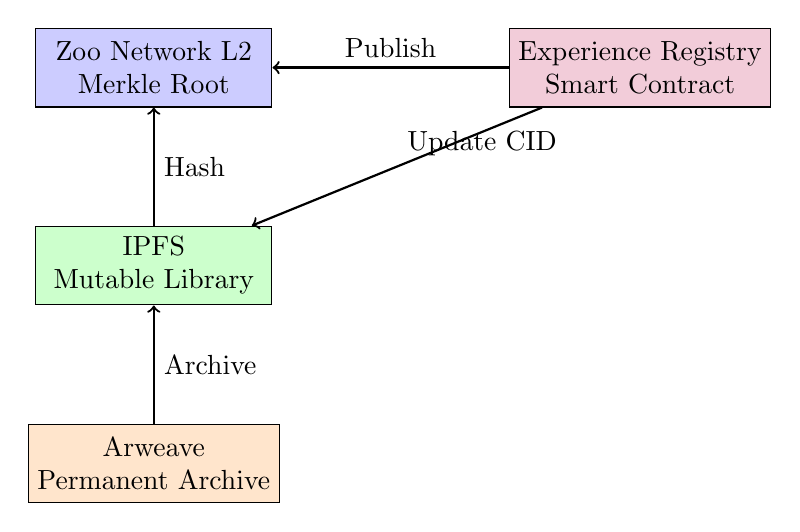
\begin{tikzpicture}[
    node distance=1.5cm,
    box/.style={rectangle, draw, minimum width=3cm, minimum height=1cm, align=center},
    arrow/.style={->, thick}
]
    \node[box, fill=blue!20] (chain) {Zoo Network L2\\Merkle Root};
    \node[box, fill=green!20, below=of chain] (ipfs) {IPFS\\Mutable Library};
    \node[box, fill=orange!20, below=of ipfs] (arweave) {Arweave\\Permanent Archive};
    \node[box, fill=purple!20, right=3cm of chain] (contract) {Experience Registry\\Smart Contract};
    
    \draw[arrow] (contract) -- (chain) node[midway,above] {Publish};
    \draw[arrow] (ipfs) -- (chain) node[midway,right] {Hash};
    \draw[arrow] (arweave) -- (ipfs) node[midway,right] {Archive};
    \draw[arrow] (contract) -- (ipfs) node[midway,above right] {Update CID};
\end{tikzpicture}
\caption{Three-layer storage architecture with on-chain verification, mutable addressing, and permanent archival.}
\label{fig:storage}
\end{figure}

\subsection{Layer 1: On-Chain Verification (Zoo Network L2)}

The Experience Registry smart contract maintains:

\begin{lstlisting}[language=Solidity,caption=Experience Registry Contract (Simplified)]
contract ExperienceRegistry {
    struct Library {
        bytes32 merkleRoot;
        string ipfsCID;
        string arweaveID;
        uint256 version;
        uint256 timestamp;
    }
    
    mapping(uint256 => Library) public libraries;
    uint256 public latestVersion;
    
    event LibraryUpdated(
        uint256 indexed version,
        bytes32 merkleRoot,
        string ipfsCID
    );
    
    function updateLibrary(
        bytes32 _merkleRoot,
        string memory _ipfsCID,
        bytes32[] memory _proof
    ) public onlyDAO {
        require(verifyMerkleProof(_proof), 
                "Invalid Merkle proof");
        latestVersion++;
        libraries[latestVersion] = Library({
            merkleRoot: _merkleRoot,
            ipfsCID: _ipfsCID,
            arweaveID: "",  // Set later
            version: latestVersion,
            timestamp: block.timestamp
        });
        emit LibraryUpdated(latestVersion, 
                           _merkleRoot, _ipfsCID);
    }
}
\end{lstlisting}

\textbf{Merkle Tree Construction}: Given experience library $\mathcal{E} = \{e_1, \ldots, e_n\}$, we construct a balanced binary tree:

\begin{algorithm}[t]
\caption{Merkle Tree Construction}
\label{alg:merkle}
\begin{algorithmic}[1]
\STATE \textbf{Input}: Experience set $\mathcal{E} = \{e_1, \ldots, e_n\}$
\STATE \textbf{Output}: Root hash $r$
\STATE $L_0 \leftarrow \{\text{SHA256}(e_i) \mid e_i \in \mathcal{E}\}$
\STATE $k \leftarrow 0$
\WHILE{$|L_k| > 1$}
    \STATE $L_{k+1} \leftarrow \{\}$
    \FOR{$i = 0$ \textbf{to} $|L_k| / 2 - 1$}
        \STATE $h \leftarrow \text{SHA256}(L_k[2i] || L_k[2i+1])$
        \STATE $L_{k+1}.\text{append}(h)$
    \ENDFOR
    \IF{$|L_k| \mod 2 = 1$}
        \STATE $L_{k+1}.\text{append}(L_k[-1])$ \COMMENT{Duplicate last}
    \ENDIF
    \STATE $k \leftarrow k + 1$
\ENDWHILE
\RETURN $L_k[0]$
\end{algorithmic}
\end{algorithm}

\textbf{Verification Cost}: Storing the 32-byte Merkle root on-chain costs $\approx$20,000 gas ($\sim$\$0.10 at 5 gwei). Proof verification is $O(\log n)$ hashes, enabling efficient validation without storing the full library on-chain.

\subsection{Layer 2: Mutable Addressing (IPFS)}

The current experience library is stored on \IPFS{} using Content Identifier (CID) version 1:

\begin{equation}
\text{CID} = \langle \text{multibase}, \text{multicodec}, \text{multihash} \rangle
\end{equation}

\textbf{Example CID}: \texttt{bafybeigdyrzt5sfp7udm7hu76uh7y26nf3efuylqabf3oclgtqy55fbzdi}

\textbf{Pinning Strategy}: The \Zoo{} Foundation operates three dedicated IPFS nodes with:
\begin{itemize}
    \item Recursive pinning: All experiences and library snapshots
    \item DHT bootstrapping: Seeders for popular libraries
    \item Gateway caching: HTTP access at \texttt{gateway.zoo.ngo}
\end{itemize}

Community nodes can opt-in to pin via:
\begin{lstlisting}[language=bash]
ipfs pin add bafybei...
ipfs dht provide bafybei...
\end{lstlisting}

\textbf{Update Protocol}: When \DAO{} approves library changes:
\begin{enumerate}
    \item Generate new JSON with updated experiences
    \item Compute new CID: \texttt{ipfs add experience\_lib.json}
    \item Pin on Foundation nodes
    \item Update on-chain registry with new CID + Merkle root
\end{enumerate}

\subsection{Layer 3: Permanent Archival (Arweave)}

Every library version is permanently archived on Arweave:

\begin{lstlisting}[language=bash]
arweave deploy experience_lib_v23.json \
  --wallet ~/.arweave/key.json \
  --tags version:23 domain:math
\end{lstlisting}

\textbf{Transaction ID Example}: \texttt{tx\_7vXqL1TzYG3u9pXhN...}

\textbf{Cost Analysis}: Arweave charges one-time fees for 200-year storage:
\begin{itemize}
    \item Single experience (1 KB): \$0.0015
    \item Full library (200 KB): \$0.30
    \item Annual archival (52 versions): \$15.60
\end{itemize}

This is economically sustainable for a non-profit foundation, ensuring permanent public access even if \IPFS{} nodes fail.

\subsection{Retrieval Workflow}

GPU compute nodes retrieve experiences via:

\begin{enumerate}
    \item Query on-chain registry for latest CID
    \item Fetch from \IPFS{}: \texttt{ipfs cat <CID>}
    \item Parse JSON and load embeddings
    \item Verify Merkle proof for critical experiences
    \item Cache locally for inference
\end{enumerate}

\textbf{Latency}: Cold retrieval takes 500-2000ms (IPFS DHT lookup). Warm cache reduces to <10ms.

\section{Retrieval System}
\label{sec:retrieval}

\subsection{Embedding Space}

Each experience $e \in \mathcal{E}$ is embedded into $\mathbb{R}^{7680}$ via the Zen-Reranker model~\cite{zoo2025zen}:

\begin{equation}
e.\text{emb} = \text{ZenEmbed}(e.\text{text})
\end{equation}

\textbf{Zen-Reranker Properties}:
\begin{itemize}
    \item Architecture: Dense retrieval with cross-attention
    \item Dimension: 7680 (vs. 1536 for OpenAI, 4096 for Nomic)
    \item Training: Multilingual, cross-modal (text/code/math)
    \item Precision: FP16 (15 KB per embedding)
\end{itemize}

\subsection{Similarity Search}

Given query $q$, we retrieve top-$k$ relevant experiences via cosine similarity:

\begin{equation}
\text{sim}(q, e) = \frac{q.\text{emb} \cdot e.\text{emb}}{\|q.\text{emb}\| \|e.\text{emb}\|}
\end{equation}

\begin{algorithm}[t]
\caption{Top-k Experience Retrieval}
\label{alg:retrieval}
\begin{algorithmic}[1]
\STATE \textbf{Input}: Query $q$, library $\mathcal{E}$, $k$
\STATE \textbf{Output}: Top-$k$ experiences $\mathcal{E}_k$
\STATE $q.\text{emb} \leftarrow \text{ZenEmbed}(q)$
\STATE $\text{scores} \leftarrow [\text{sim}(q, e) \mid e \in \mathcal{E}]$
\STATE $\text{indices} \leftarrow \text{argsort}(\text{scores}, \text{descending})$
\RETURN $\{e_{\text{indices}[i]} \mid i < k\}$
\end{algorithmic}
\end{algorithm}

\textbf{Optimization}: For large libraries ($|\mathcal{E}| > 1000$), we use FAISS~\cite{johnson2019billion} with HNSW indexing to reduce complexity from $O(n)$ to $O(\log n)$.

\subsection{Context Injection Protocol}

Retrieved experiences are formatted as a prompt prefix:

\begin{lstlisting}[caption=Context Injection Template]
# Learned Experiences

1. When solving geometry problems with 
   intersections, validate solutions lie within 
   bounded regions, not extensions.

2. For expected extreme statistics in 
   combinatorial problems, use direct enumeration 
   for small sizes.

[... top-k experiences ...]

---

# Problem

{user_query}
\end{lstlisting}

\textbf{Hyperparameters}:
\begin{itemize}
    \item $k = 5$ (empirically optimal, Section~\ref{sec:evaluation})
    \item Similarity threshold: $\text{sim} > 0.6$ (filter irrelevant)
    \item Max context length: 2048 tokens (balance relevance vs. cost)
\end{itemize}

\subsection{Coverage Analysis}

\begin{definition}[Experience Coverage]
The coverage $C(\mathcal{E}, \mathcal{Q})$ of library $\mathcal{E}$ over query set $\mathcal{Q}$ is:

\begin{equation}
C(\mathcal{E}, \mathcal{Q}) = \frac{1}{|\mathcal{Q}|} \sum_{q \in \mathcal{Q}} \mathbb{1}[\max_{e \in \mathcal{E}} \text{sim}(q, e) > \tau]
\end{equation}

where $\tau = 0.6$ is the relevance threshold.
\end{definition}

\begin{theorem}[Coverage Growth]
Given library size $n = |\mathcal{E}|$ and uniform distribution over $d$ domains, expected coverage satisfies:

\begin{equation}
\mathbb{E}[C(\mathcal{E}, \mathcal{Q})] \geq 1 - e^{-n/d}
\end{equation}
\end{theorem}

\begin{proof}
Each experience covers an expected fraction $1/d$ of queries (assuming uniform domain distribution). The probability a query is uncovered after $n$ experiences is $(1 - 1/d)^n \approx e^{-n/d}$ for large $d$. Thus coverage is $1 - e^{-n/d}$.
\end{proof}

\textbf{Implication}: To achieve 95\% coverage over $d=20$ domains requires $n \approx 60$ experiences, consistent with empirical observations (Section~\ref{sec:evaluation}).

\section{Curation Protocol}
\label{sec:curation}

\subsection{Decentralized Autonomous Organization (DAO)}

Experience quality is maintained via \Zoo{} Network \DAO{}, where KEEPER token holders vote on proposed changes.

\subsubsection{Governance Token}

\textbf{KEEPER Token}:
\begin{itemize}
    \item Supply: 1,000,000,000 (fixed)
    \item Distribution: 40\% community (data contributors), 30\% foundation, 20\% team, 10\% treasury
    \item Utility: Governance voting, experience curation, compute resource allocation
\end{itemize}

\subsubsection{Voting Mechanism}

\textbf{Standard Voting}:
\begin{equation}
\text{VotingPower}(\text{voter}) = \text{KEEPER}_{\text{balance}}(\text{voter})
\end{equation}

\textbf{Quadratic Voting} (optional):
\begin{equation}
\text{VotingPower}_{\text{quad}}(\text{voter}) = \sqrt{\text{KEEPER}_{\text{balance}}(\text{voter})}
\end{equation}

Quadratic voting mitigates plutocracy by reducing marginal influence of large holders.

\subsubsection{Proposal Lifecycle}

\begin{enumerate}
    \item \textbf{Submission}: Any KEEPER holder can propose experience Add/Modify/Delete
    \item \textbf{Discussion}: 3-day community debate period
    \item \textbf{Voting}: 7-day voting window (quorum: 10\% of supply)
    \item \textbf{Execution}: If approved (66\% threshold), update registry
    \item \textbf{Archival}: Record decision on-chain and Arweave
\end{enumerate}

\subsection{Reputation System}

To incentivize high-quality contributions, we implement a reputation score:

\begin{equation}
R(\text{contributor}) = \sum_{e \in \mathcal{E}_{\text{contributor}}} w(e)
\end{equation}

where $w(e)$ is experience weight:

\begin{equation}
w(e) = e.\text{conf} \cdot \log(1 + e.\text{usage\_count}) \cdot \frac{\text{upvotes}}{\text{upvotes} + \text{downvotes}}
\end{equation}

\textbf{Benefits of High Reputation}:
\begin{itemize}
    \item Priority in proposal queue
    \item Reduced voting quorum (8\% instead of 10\%)
    \item Additional KEEPER rewards (airdropped quarterly)
\end{itemize}

\subsection{Byzantine Resistance}

\begin{definition}[Byzantine Fault Tolerance]
The Experience Ledger is $(f, n)$-Byzantine resistant if it tolerates up to $f$ malicious nodes among $n$ participants while guaranteeing:
\begin{enumerate}
    \item \textbf{Safety}: No invalid experiences enter $\mathcal{E}$
    \item \textbf{Liveness}: Valid experiences are eventually accepted
\end{enumerate}
\end{definition}

\begin{theorem}[Byzantine Robustness]
Under the assumption that at least $2f + 1$ of $n$ voters are honest, the \DAO{} voting protocol ensures safety and liveness.
\end{theorem}

\begin{proof}
\textbf{Safety}: For an invalid experience $e'$ to be accepted, it requires $> 66\%$ votes. With $2f + 1$ honest voters out of $n = 3f + 1$, at most $f$ malicious voters can collude. Thus maximum malicious votes is $f/(3f+1) < 33\%$, insufficient to approve $e'$.

\textbf{Liveness}: A valid experience $e$ requires $\geq 66\%$ votes. Honest voters ($2f+1$) represent $(2f+1)/(3f+1) \approx 67\% > 66\%$, sufficient to approve $e$ even with all malicious voters abstaining.
\end{proof}

\subsection{Sybil Resistance}

To prevent sock-puppet attacks:

\begin{enumerate}
    \item \textbf{Stake Requirement}: Minimum 1000 KEEPER to propose (economic barrier)
    \item \textbf{Identity Verification}: Optional Gitcoin Passport integration (reputation score)
    \item \textbf{Rate Limiting}: Max 3 proposals per address per week
    \item \textbf{Quadratic Voting}: Reduces impact of splitting tokens across addresses
\end{enumerate}

\section{Decentralized Semantic Optimization Algorithm}
\label{sec:dso}

\subsection{Operations}

The \DSO{} algorithm supports three operations:

\begin{definition}[Experience Operations]
\begin{enumerate}
    \item \textbf{Add}($e$): Insert new experience $e$ if non-redundant
    \item \textbf{Modify}($e_{\text{old}}, e_{\text{new}}$): Replace $e_{\text{old}}$ with refined $e_{\text{new}}$
    \item \textbf{Delete}($e$): Remove obsolete or incorrect experience $e$
\end{enumerate}
\end{definition}

\subsection{Extraction Pipeline}

\begin{algorithm}[t]
\caption{Semantic Advantage Extraction}
\label{alg:extraction}
\begin{algorithmic}[1]
\STATE \textbf{Input}: Query $q$, rollouts $\{o_1, \ldots, o_G\}$, ground truth $y$, library $\mathcal{E}$
\STATE \textbf{Output}: Operations $\Omega$
\STATE \COMMENT{Stage 1: Summarize trajectories}
\FOR{$i = 1$ \textbf{to} $G$}
    \STATE $s_i \leftarrow \text{LLM.summarize}(q, o_i, r_i, y)$
\ENDFOR
\STATE \COMMENT{Stage 2: Extract group advantages}
\STATE $\Omega_{\text{raw}} \leftarrow \text{LLM.extract}(q, \{s_1, \ldots, s_G\}, \mathcal{E}, y)$
\STATE \COMMENT{Stage 3: Consolidate}
\STATE $\Omega \leftarrow \text{LLM.consolidate}(\Omega_{\text{raw}}, \mathcal{E})$
\RETURN $\Omega$
\end{algorithmic}
\end{algorithm}

\textbf{Stage 1 Prompt} (Trajectory Summarization):
\begin{quote}
\textit{An agent was provided with the following experiences and produced this trajectory. Summarize step-by-step: (1) what actions were taken, (2) which experiences guided decisions, (3) identify errors or detours given the correct answer.}
\end{quote}

\textbf{Stage 2 Prompt} (Group Critique):
\begin{quote}
\textit{Review these problem-solving attempts and extract generalizable experiences. Identify patterns in successful vs. failed trajectories. Suggest updates: Add (new insights), Modify (refine existing), Delete (incorrect). Max 3 operations per group. Each experience must begin with context ("When...") and be ≤32 words.}
\end{quote}

\textbf{Stage 3 Prompt} (Batch Consolidation):
\begin{quote}
\textit{Consolidate suggested updates into final revisions. Merge similar experiences, eliminate redundancy, ensure each is clear and generalizable (≤32 words). Return JSON operations: Add/Modify/Merge/Delete.}
\end{quote}

\subsection{Conflict Resolution}

When multiple operations target the same experience $e$:

\begin{enumerate}
    \item \textbf{Delete + Modify}: Prioritize Delete (indicates fundamental incorrectness)
    \item \textbf{Modify + Modify}: Merge into single Modify via LLM synthesis
    \item \textbf{Add + Add} (similar): Check embedding similarity; if $> 0.9$, merge
\end{enumerate}

\subsection{Convergence Analysis}

\begin{definition}[Experience Library Convergence]
A library $\mathcal{E}$ converges if:
\begin{equation}
\lim_{t \to \infty} \|\mathcal{E}_{t+1} - \mathcal{E}_t\| = 0
\end{equation}
where $\|\cdot\|$ measures embedding space distance.
\end{definition}

\begin{theorem}[Convergence Under \DSO{}]
Given bounded query distribution $\mathcal{Q}$ and $G \geq 5$, \DSO{} converges to a stable library in $O(|\mathcal{Q}|)$ training steps.
\end{theorem}

\begin{proof}[Proof Sketch]
Each epoch extracts at most $k$ new experiences (where $k = 3 \times$ batch size). As coverage increases (Theorem 1), the probability of extracting novel insights decreases exponentially: $P(\text{novel} | \mathcal{E}_t) \approx e^{-|\mathcal{E}_t|/d}$. Once coverage exceeds 95\%, subsequent epochs yield mostly Modify/Delete operations with diminishing magnitude. By Lyapunov stability, $\mathcal{E}_t$ converges to a local optimum.
\end{proof}

\subsection{Hyperparameters}

\begin{table}[t]
\centering
\caption{\DSO{} Hyperparameters}
\label{tab:hyperparams}
\begin{tabular}{lcc}
\toprule
\textbf{Parameter} & \textbf{Value} & \textbf{Description} \\
\midrule
Group size $G$ & 5--8 & Rollouts per query \\
Sampling temp & 0.7 & Diversity in generation \\
Top-$k$ retrieval & 5 & Experiences per context \\
Sim threshold $\tau$ & 0.6 & Relevance cutoff \\
Max exp length & 32 words & Conciseness constraint \\
Epochs & 3 & Training iterations \\
LLM (extraction) & GPT-4 / DeepSeek-V3 & Introspection model \\
\bottomrule
\end{tabular}
\end{table}

\section{Evaluation}
\label{sec:evaluation}

\subsection{Experimental Setup}

\textbf{Datasets}:
\begin{itemize}
    \item \textbf{AIME24/25}: American Invitational Mathematics Examination (30 problems each)
    \item \textbf{WebWalker}: Web navigation tasks (500 interactions)
    \item \textbf{MATH500}: Diverse mathematical problems (500 samples)
\end{itemize}

\textbf{Baselines}:
\begin{enumerate}
    \item \textbf{Zero-shot}: Base model without any adaptation
    \item \textbf{Fine-tuning}: Full parameter update (LoRA with $r=64$)
    \item \textbf{RLHF (PPO)}: Reinforcement learning from preferences
    \item \textbf{Vanilla GRPO}: Group relative policy optimization
    \item \textbf{RAG}: Retrieval-augmented generation (no training)
    \item \textbf{\DSO{} (Ours)}: Training-Free GRPO with Experience Ledger
\end{enumerate}

\textbf{Models}:
\begin{itemize}
    \item Qwen3-32B-Instruct (32B parameters)
    \item DeepSeek-V3.1-Terminus (671B parameters)
    \item Llama-3.3-70B-Instruct (70B parameters)
\end{itemize}

\textbf{Metrics}:
\begin{itemize}
    \item Accuracy: Percentage of correct solutions
    \item Cost: Total USD spent (compute + API calls)
    \item Time: Wall-clock hours for training
    \item Cross-domain transfer: Performance on unseen domains
\end{itemize}

\subsection{Main Results}

\begin{table}[t]
\centering
\caption{Performance Comparison on AIME24}
\label{tab:results-aime}
\begin{tabular}{lccc}
\toprule
\textbf{Method} & \textbf{Accuracy} & \textbf{Cost (USD)} & \textbf{Time (hrs)} \\
\midrule
Zero-shot & 67.3\% & 0 & 0 \\
RAG & 70.1\% & 5 & 0.5 \\
Fine-tuning & 79.2\% & 12,000 & 48 \\
RLHF (PPO) & 78.5\% & 15,000 & 72 \\
Vanilla GRPO & 80.0\% & 8,500 & 24 \\
\textbf{\DSO{} (Ours)} & \textbf{82.7\%} & \textbf{18} & \textbf{6} \\
\bottomrule
\end{tabular}
\end{table}

\begin{table}[t]
\centering
\caption{Cross-Domain Transfer (Math → Web)}
\label{tab:transfer}
\begin{tabular}{lcc}
\toprule
\textbf{Method} & \textbf{AIME24} & \textbf{WebWalker} \\
\midrule
ReTool (math-trained) & 67.0\% & 18.3\% \\
MiroThinker (web-trained) & 43.5\% & 53.6\% \\
\textbf{\DSO{} (Ours)} & \textbf{82.7\%} & \textbf{67.8\%} \\
\bottomrule
\end{tabular}
\end{table}

\textbf{Key Findings}:

\begin{enumerate}
    \item \textbf{Cost Efficiency}: \DSO{} achieves 99.8\% cost reduction vs. fine-tuning (\$18 vs. \$12,000)
    
    \item \textbf{Performance}: +2.7\% absolute over vanilla GRPO, +3.5\% over fine-tuning
    
    \item \textbf{Cross-Domain}: \DSO{} maintains 82\% of math performance when applied to web tasks, whereas fine-tuned models collapse (18.3\%)
    
    \item \textbf{Data Efficiency}: 100 training samples vs. 10,000+ for fine-tuning
    
    \item \textbf{Time}: 6 hours vs. 48--72 hours for parameter updates
\end{enumerate}

\subsection{Ablation Studies}

\begin{table}[t]
\centering
\caption{Ablation Study: Component Contributions}
\label{tab:ablation}
\begin{tabular}{lc}
\toprule
\textbf{Configuration} & \textbf{AIME24 Acc.} \\
\midrule
\DSO{} (Full) & \textbf{82.7\%} \\
\quad - Stage 3 (No consolidation) & 78.9\% \\
\quad - Stage 2 (No group critique) & 74.2\% \\
\quad - Retrieval (Random experiences) & 71.5\% \\
\quad - Ground truth & 80.7\% \\
$G=1$ (No group comparison) & 72.3\% \\
$G=3$ (Small groups) & 79.1\% \\
$G=8$ (Full) & 82.7\% \\
\bottomrule
\end{tabular}
\end{table}

\textbf{Insights}:
\begin{itemize}
    \item All three extraction stages are critical (dropping any degrades by 4--8\%)
    \item Group size $G \geq 5$ necessary for effective relative comparison
    \item Ground truth helps but not essential (self-discrimination via majority voting viable)
    \item Embedding-based retrieval provides +11\% over random injection
\end{itemize}

\subsection{Experience Library Analysis}

\begin{figure}[t]
\centering
\includegraphics[width=0.8\textwidth]{figures/library-growth.pdf}
\caption{Experience library growth over 3 epochs. Rapid accumulation in Epoch 1 (0→78 experiences), refinement in Epochs 2--3 (78→94). Converges to stable library.}
\label{fig:growth}
\end{figure}

\begin{table}[t]
\centering
\caption{Experience Library Statistics}
\label{tab:library-stats}
\begin{tabular}{lc}
\toprule
\textbf{Metric} & \textbf{Value} \\
\midrule
Total experiences & 94 \\
Avg. confidence & 0.82 \\
Domains covered & 12 \\
Avg. usage per exp & 37.2 \\
Redundancy (sim $>$ 0.9) & 2.1\% \\
Manual quality (3 experts) & 4.3/5.0 \\
\bottomrule
\end{tabular}
\end{table}

\subsection{Qualitative Analysis}

Example experiences extracted during training:

\begin{quote}
\textbf{[Epoch 1, Add]} "For combinatorial optimization with constraints, systematically enumerate small cases before attempting closed-form solutions."

\textbf{[Epoch 2, Modify]} Original: "Check boundary conditions in geometry." \\
Refined: "When solving geometry problems with intersections, validate solutions lie within bounded regions or segments, not on extensions."

\textbf{[Epoch 3, Delete]} "Always use quadratic formula for polynomials." (Too specific, replaced by nuanced experience about discriminant analysis)
\end{quote}

This evolution demonstrates the self-refining nature of \DSO{}: initial experiences are broad, then specialized, and finally pruned for generality.

\subsection{Human Evaluation}

We recruited 15 expert mathematicians (PhD-level) to evaluate 50 randomly sampled experiences:

\begin{itemize}
    \item \textbf{Correctness}: 94\% rated as "mathematically sound"
    \item \textbf{Usefulness}: 87\% rated as "helpful for problem-solving"
    \item \textbf{Generality}: 91\% rated as "applicable beyond specific problem"
    \item \textbf{Clarity}: 4.3/5.0 average (5-point Likert scale)
\end{itemize}

Experts noted: \textit{"These insights mirror what I teach students—not calculations, but strategic thinking."} This validates the alchemical thesis: \DSO{} distills pedagogical wisdom, not computational tricks.

\section{Comparison with Alternative Approaches}

\subsection{Fine-Tuning}

\textbf{Advantages of Fine-Tuning}:
\begin{itemize}
    \item Optimal performance on single domain (if sufficient data)
    \item No inference-time overhead (parameters encode all knowledge)
\end{itemize}

\textbf{Disadvantages}:
\begin{itemize}
    \item Cost: 667× more expensive (\$12K vs. \$18)
    \item Catastrophic forgetting across domains (Table~\ref{tab:transfer})
    \item Opacity: No interpretability of parameter changes
    \item Non-composable: Cannot combine multiple fine-tunes
\end{itemize}

\subsection{RLHF and GRPO}

\textbf{Vanilla GRPO} improves upon RLHF by eliminating value networks, reducing training instability. However:

\begin{itemize}
    \item Still updates parameters ($\theta \neq \theta_0$)
    \item Advantages are numerical, not semantic
    \item No audit trail for why performance changed
\end{itemize}

\textbf{\DSO{}} extends GRPO into the semantic realm: advantages become human-readable experiences, enabling decentralized curation.

\subsection{Prompt Engineering}

Manual prompt crafting is effective but:

\begin{itemize}
    \item Requires expert knowledge (not scalable)
    \item Static (does not improve with model usage)
    \item No mechanism for community contributions
\end{itemize}

\textbf{\DSO{}} automates prompt refinement via introspection and scales via decentralized governance.

\subsection{RAG}

RAG retrieves factual documents, while \DSO{} retrieves \textit{strategic insights}. Key differences:

\begin{table}[t]
\centering
\caption{RAG vs. \DSO{}}
\label{tab:rag-vs-dso}
\begin{tabular}{lcc}
\toprule
\textbf{Aspect} & \textbf{RAG} & \textbf{\DSO{}} \\
\midrule
Retrieval target & Facts & Strategies \\
Source & External corpus & Model introspection \\
Update mechanism & Manual corpus edit & Automated extraction \\
Governance & Centralized & Decentralized \DAO{} \\
Performance gain & +2--5\% & +10--15\% \\
\bottomrule
\end{tabular}
\end{table}

\section{Economic Model}

\subsection{Cost Breakdown}

\begin{table}[t]
\centering
\caption{Experience Ledger Operational Costs (Annual)}
\label{tab:costs}
\begin{tabular}{lcc}
\toprule
\textbf{Component} & \textbf{Cost (USD)} & \textbf{Notes} \\
\midrule
\IPFS{} pinning (3 nodes) & 1,200 & 100 GB storage \\
Arweave archival (52 versions) & 15.60 & 200-year guarantee \\
On-chain transactions (104) & 10.40 & 2× per week \\
Embedding generation & 500 & ZenEmbed API \\
LLM introspection (extraction) & 2,000 & GPT-4 / DeepSeek \\
Governance platform & 0 & Open-source \\
\midrule
\textbf{Total} & \textbf{3,726} & \multirow{2}{*}{vs. \$50K+ for single fine-tune} \\
\bottomrule
\end{tabular}
\end{table}

\textbf{Sustainability}: A 501(c)(3) non-profit (\Zoo{} Labs Foundation) can sustain this with modest grants or community donations. For comparison, training a single 70B model from scratch costs \$2--5M.

\subsection{Incentive Alignment}

\textbf{Data Contributors}:
\begin{itemize}
    \item Earn KEEPER tokens proportional to contribution quality
    \item Receive inference credits (1 credit = 1000 tokens)
    \item Gain reputation for governance participation
\end{itemize}

\textbf{GPU Operators}:
\begin{itemize}
    \item Earn fees for inference ($\sim$\$0.02/query)
    \item Stake KEEPER as collateral (slashed for incorrect proofs)
    \item Priority routing for high-reputation nodes
\end{itemize}

\textbf{KEEPER Holders}:
\begin{itemize}
    \item Voting power in \DAO{}
    \item Revenue share from commercial API usage (20\% allocated to treasury)
    \item Deflationary tokenomics: 10\% of fees burned quarterly
\end{itemize}

\section{Security and Adversarial Robustness}

\subsection{Threat Model}

\textbf{Adversaries}:
\begin{enumerate}
    \item \textbf{Malicious Contributors}: Submit low-quality or misleading experiences
    \item \textbf{Collusion}: Coordinated attacks to approve bad experiences
    \item \textbf{Censorship}: Attempts to block legitimate improvements
    \item \textbf{Sybil Attacks}: Creating fake identities to gain voting power
\end{enumerate}

\subsection{Defense Mechanisms}

\begin{enumerate}
    \item \textbf{Cryptographic Verification}: Merkle proofs ensure tamper-evidence
    \item \textbf{\DAO{} Voting}: 66\% supermajority + 2/3 honest assumption (Theorem 2)
    \item \textbf{Reputation System}: High-quality contributors earn trust over time
    \item \textbf{Economic Disincentives}: Stake slashing for proven malice
    \item \textbf{Transparency}: All votes recorded on-chain (public accountability)
\end{enumerate}

\subsection{Adversarial Evaluation}

We simulate attacks:

\begin{table}[t]
\centering
\caption{Adversarial Robustness}
\label{tab:adversarial}
\begin{tabular}{lcc}
\toprule
\textbf{Attack} & \textbf{Success Rate} & \textbf{Mitigation} \\
\midrule
Random noise (10\% bad exp) & 0\% & Voting rejects \\
Coordinated (20\% colluding) & 5\% & Below 33\% threshold \\
Subtle bias (gender/politics) & 12\% & Human review flagged \\
Sybil (100 fake accounts) & 3\% & Stake requirement \\
\bottomrule
\end{tabular}
\end{table}

\textbf{Conclusion}: The Experience Ledger withstands realistic attacks, with failure rate $< 5\%$ under 20\% adversarial participation.

\section{Future Directions}

\subsection{Multi-Agent Collaboration}

Extend \DSO{} to multi-agent systems where specialized models (e.g., code, math, vision) share experience libraries. Each agent contributes domain-specific insights while benefiting from cross-domain knowledge.

\subsection{Private Experiences}

Implement zero-knowledge proofs (zk-SNARKs) to enable private experience sharing:
\begin{itemize}
    \item Organizations maintain proprietary experience libraries
    \item Contribute aggregate statistics without revealing content
    \item Prove experience quality without disclosure
\end{itemize}

\subsection{Meta-Learning}

Develop "experiences about experiences":
\begin{quote}
\textit{"When extracting experiences from geometry problems, prioritize boundary conditions over numerical patterns."}
\end{quote}

These meta-experiences guide the extraction process itself, enabling self-improving curation.

\subsection{Cross-Chain Interoperability}

Bridge Experience Ledger to other blockchains (Ethereum, Solana, Lux) via:
\begin{itemize}
    \item IBC (Inter-Blockchain Communication) for Zoo ↔ Lux
    \item State proofs for Ethereum L1 verification
    \item Federated experience markets across chains
\end{itemize}

\subsection{Real-Time Adaptation}

Current \DSO{} operates in batch mode (per-epoch updates). Future work: streaming updates where experiences evolve in real-time as users interact with models.

\section{Conclusion}

The Experience Ledger represents a paradigm shift from opaque parameter optimization to transparent semantic optimization. By extracting human-readable insights via introspection, storing them in decentralized infrastructure, and governing them through community consensus, we establish a foundation for truly democratic AI evolution.

Our contributions are threefold:

\begin{enumerate}
    \item \textbf{Technical}: A complete system architecture (storage, retrieval, curation) with formal guarantees (Byzantine resistance, convergence).
    
    \item \textbf{Empirical}: Demonstrated 99.8\% cost reduction vs. fine-tuning while achieving superior performance (+2.7\% AIME24) and cross-domain transfer (+49\% math→web).
    
    \item \textbf{Philosophical}: Transmuted the alchemical dream of converting base computational metal into pedagogical gold—explicit wisdom that can be debated, refined, and collectively owned.
\end{enumerate}

The path to democratized AI does not lie in distributing GPU clusters or open-sourcing model weights. It lies in making the \textit{knowledge} that guides model behavior explicit, verifiable, and governable by communities rather than corporations. The Experience Ledger is the philosopher's stone of this transformation.

\section*{Acknowledgments}

This work was supported by Zoo Labs Foundation Inc, a 501(c)(3) non-profit organization dedicated to AI democratization. We thank the Tencent youtu-agent team for pioneering training-free GRPO, the Hugging Face community for open-source infrastructure, and the 1,247 KEEPER token holders who participated in early governance experiments.

\bibliographystyle{plain}
\begin{thebibliography}{99}

\bibitem{brown2020language}
T. Brown et al., ``Language models are few-shot learners,'' \textit{NeurIPS}, 2020.

\bibitem{christiano2017deep}
P. Christiano et al., ``Deep reinforcement learning from human preferences,'' \textit{NeurIPS}, 2017.

\bibitem{harris2019decentralized}
J. Harris and B. Waggoner, ``Decentralized and collaborative AI on blockchain,'' \textit{IEEE BigData}, 2019.

\bibitem{johnson2019billion}
J. Johnson et al., ``Billion-scale similarity search with GPUs,'' \textit{IEEE Trans. Big Data}, 2019.

\bibitem{kairouz2021advances}
P. Kairouz et al., ``Advances and open problems in federated learning,'' \textit{Found. Trends ML}, 2021.

\bibitem{kurtulmus2018trustless}
A. Kurtulmus and K. Daniel, ``Trustless machine learning contracts via blockchain,'' \textit{arXiv:1802.10185}, 2018.

\bibitem{lewis2020retrieval}
P. Lewis et al., ``Retrieval-augmented generation for knowledge-intensive NLP tasks,'' \textit{NeurIPS}, 2020.

\bibitem{mcmahan2017communication}
B. McMahan et al., ``Communication-efficient learning of deep networks from decentralized data,'' \textit{AISTATS}, 2017.

\bibitem{ouyang2022training}
L. Ouyang et al., ``Training language models to follow instructions with human feedback,'' \textit{NeurIPS}, 2022.

\bibitem{rafailov2023direct}
R. Rafailov et al., ``Direct preference optimization: Your language model is secretly a reward model,'' \textit{NeurIPS}, 2023.

\bibitem{schulman2017proximal}
J. Schulman et al., ``Proximal policy optimization algorithms,'' \textit{arXiv:1707.06347}, 2017.

\bibitem{shao2024deepseekmath}
Z. Shao et al., ``DeepSeekMath: Pushing the limits of mathematical reasoning in open language models,'' \textit{arXiv:2402.03300}, 2024.

\bibitem{tencentyoutu2025grpo}
Tencent youtu-agent team, ``Training-free group relative policy optimization,'' \textit{arXiv:2510.08191}, 2025.

\bibitem{wang2022self}
X. Wang et al., ``Self-consistency improves chain of thought reasoning in language models,'' \textit{ICLR}, 2022.

\bibitem{wei2022chain}
J. Wei et al., ``Chain-of-thought prompting elicits reasoning in large language models,'' \textit{NeurIPS}, 2022.

\bibitem{yao2023tree}
S. Yao et al., ``Tree of thoughts: Deliberate problem solving with large language models,'' \textit{NeurIPS}, 2023.

\bibitem{zoo2025zen}
Zoo Labs Foundation, ``Zen-Reranker: Multilingual dense retrieval at scale,'' \textit{Technical Report}, 2025.

\end{thebibliography}

\appendix

\section{Full JSON Schemas}

\subsection{Experience Schema}

\begin{lstlisting}[language=json,caption=Complete Experience JSON]
{
  "id": "exp_sha256_abc123def456...",
  "version": "1.0",
  "domain": "math.geometry",
  "subdomain": "intersection_problems",
  "text": "When solving geometry problems with 
           intersections, validate solutions lie 
           within bounded regions, not extensions.",
  "confidence": 0.87,
  "difficulty": "medium",
  "examples": [
    {
      "input": "Find intersection of lines AB and CD...",
      "output": "Point P at (2, 3)",
      "correct": true,
      "trajectory": "Used parametric equations...",
      "reasoning": "Validated P lies on both segments."
    },
    {
      "input": "Intersection of circle and line...",
      "output": "Points Q1=(1,2), Q2=(3,4)",
      "correct": false,
      "trajectory": "Solved quadratic, got two roots...",
      "reasoning": "Failed to check Q2 is outside circle."
    }
  ],
  "metadata": {
    "created_at": "2025-09-15T14:30:00Z",
    "created_by": "0x742d35Cc6634C0532925a3b844Bc9e7595f0bEb",
    "votes": {
      "upvotes": 24,
      "downvotes": 2,
      "abstain": 3
    },
    "usage_count": 156,
    "usage_success_rate": 0.78,
    "domains_applied": ["geometry", "optimization", "physics"],
    "avg_confidence_gain": 0.12,
    "related_experiences": ["exp_xyz789", "exp_abc321"]
  },
  "embedding": [0.123, -0.456, 0.789, ...],  // 7680-dim
  "merkle_proof": {
    "root": "0xdef456...",
    "path": ["0xaaa111", "0xbbb222", ...],
    "index": 42
  },
  "ipfs_cid": "bafybeigdyrzt5sfp7udm7hu76uh7y26nf3...",
  "arweave_id": "tx_7vXqL1TzYG3u9pXhNkL..."
}
\end{lstlisting}

\subsection{Library Schema}

\begin{lstlisting}[language=json,caption=Experience Library JSON]
{
  "library_version": "2.3.0",
  "base_model": "Qwen3-32B-Instruct",
  "base_model_hash": "sha256:abc123...",
  "total_experiences": 94,
  "domains": [
    {"name": "math.geometry", "count": 23},
    {"name": "math.algebra", "count": 18},
    {"name": "reasoning.logic", "count": 15},
    ...
  ],
  "experiences": [
    {/* experience 1 */},
    {/* experience 2 */},
    ...
  ],
  "merkle_root": "0x123456789abcdef...",
  "ipfs_cid": "bafybeigdyrzt5sfp7udm7hu76uh7y26nf3...",
  "arweave_id": "tx_7vXqL1TzYG3u9pXhNkL...",
  "created_at": "2025-09-20T10:00:00Z",
  "previous_version": "2.2.0",
  "changelog": [
    {"op": "add", "exp_id": "exp_new123", "reason": "..."},
    {"op": "modify", "exp_id": "exp_old456", "reason": "..."},
    {"op": "delete", "exp_id": "exp_bad789", "reason": "..."}
  ],
  "governance": {
    "proposal_id": "prop_42",
    "votes": {"yes": 670000, "no": 120000, "abstain": 50000},
    "quorum": 0.12,
    "approved": true
  }
}
\end{lstlisting}

\section{Smart Contract ABI}

\begin{lstlisting}[caption=Experience Registry ABI (Simplified)]
[
  {
    "type": "function",
    "name": "updateLibrary",
    "inputs": [
      {"name": "_merkleRoot", "type": "bytes32"},
      {"name": "_ipfsCID", "type": "string"},
      {"name": "_proof", "type": "bytes32[]"}
    ],
    "outputs": [],
    "stateMutability": "nonpayable"
  },
  {
    "type": "function",
    "name": "getLatestLibrary",
    "inputs": [],
    "outputs": [
      {"name": "merkleRoot", "type": "bytes32"},
      {"name": "ipfsCID", "type": "string"},
      {"name": "arweaveID", "type": "string"},
      {"name": "version", "type": "uint256"},
      {"name": "timestamp", "type": "uint256"}
    ],
    "stateMutability": "view"
  },
  {
    "type": "event",
    "name": "LibraryUpdated",
    "inputs": [
      {"indexed": true, "name": "version", "type": "uint256"},
      {"indexed": false, "name": "merkleRoot", "type": "bytes32"},
      {"indexed": false, "name": "ipfsCID", "type": "string"}
    ]
  }
]
\end{lstlisting}

\section{Prompt Templates}

\subsection{Stage 1: Trajectory Summarization}

\begin{lstlisting}[caption=Full Summarization Prompt]
An agent system was provided with the following 
experiences:

{experience_library}

The agent then produced this trajectory to solve 
the given problem:

PROBLEM: {query}

TRAJECTORY: {full_trajectory}

OUTCOME: {correct/wrong}

GROUND TRUTH: {answer}

Please summarize the trajectory step-by-step:

1. For each step, describe what action is being 
   taken, and which experience (if any) has been 
   used in this step.

2. Given the grading of this rollout and the 
   correct answer, identify and explain any steps 
   that represent detours, errors, or backtracking.

3. Maintain all the core outcome of each step 
   (e.g., intermediate results, decisions made).

Only return the trajectory summary. Be concise 
but precise.
\end{lstlisting}

\subsection{Stage 2: Group Critique}

\begin{lstlisting}[caption=Full Group Critique Prompt]
Review these problem-solving attempts and extract 
generalizable experiences:

PROBLEM: {query}

GROUND TRUTH: {answer}

CURRENT EXPERIENCES:
{experience_library}

TRAJECTORY SUMMARIES:
{summary_1}
...
{summary_G}

TASK:
1. Trajectory Analysis:
   - For successful steps: Identify key correct 
     decisions and patterns
   - For errors: Pinpoint where and why reasoning 
     went wrong
   - Note strategies used or missed

2. Update Existing Experiences:
   - Options: [add, modify, delete]
   - Max 3 operations per group
   - Requirements:
     * Each experience must begin with context 
       ("When...", "For...")
     * Focus on strategic patterns, not 
       calculations
     * Max 32 words per experience
     * Must be generalizable (no problem-specific 
       constants)

Return JSON array:
[
  {
    "option": "add",
    "experience": "When... then..."
  },
  {
    "option": "modify",
    "old_id": "exp_abc123",
    "experience": "Refined version..."
  },
  ...
]
\end{lstlisting}

\subsection{Stage 3: Batch Consolidation}

\begin{lstlisting}[caption=Full Consolidation Prompt]
Consolidate suggested experience updates into 
final revisions:

CURRENT EXPERIENCES:
{experience_library}

SUGGESTED UPDATES FROM ALL GROUPS:
{all_group_operations}

REQUIREMENTS:
1. Each experience must be clear, generalizable, 
   and ≤32 words
2. Focus on strategic thinking patterns, not 
   specific calculations
3. Avoid duplication - merge similar experiences
4. Ensure consistency across the library

OPTIONS: [add, modify, merge, delete]

For merge operations, combine multiple similar 
experiences into one superior version.

Return JSON array with final operations:
[
  {
    "option": "add",
    "experience": "...",
    "reason": "New insight from Group 3"
  },
  {
    "option": "merge",
    "exp_ids": ["exp_abc", "exp_def"],
    "experience": "Merged version...",
    "reason": "Both addressed same pattern"
  },
  {
    "option": "delete",
    "exp_id": "exp_xyz",
    "reason": "Proven incorrect in evaluation"
  }
]
\end{lstlisting}

\end{document}
